\documentclass[tikz,border=4pt]{standalone}
% Shared setup for the foundation-model diagrams, in the AFRICAST palette
\usepackage{fontspec}
\usepackage[sfdefault]{FiraSans}
\usepackage{amsmath}
\usepackage{unicode-math}
\setmathfont{Fira Math}
\usetikzlibrary{arrows.meta}
\definecolor{ink}{HTML}{1F2A36}
\definecolor{MonashBlue}{HTML}{3B75AC}
\definecolor{Orange}{HTML}{B5570F}
\color{ink}
\tikzset{every picture/.style={draw=ink,>=stealth}}
\hyphenpenalty=10000
\exhyphenpenalty=10000

\begin{document}
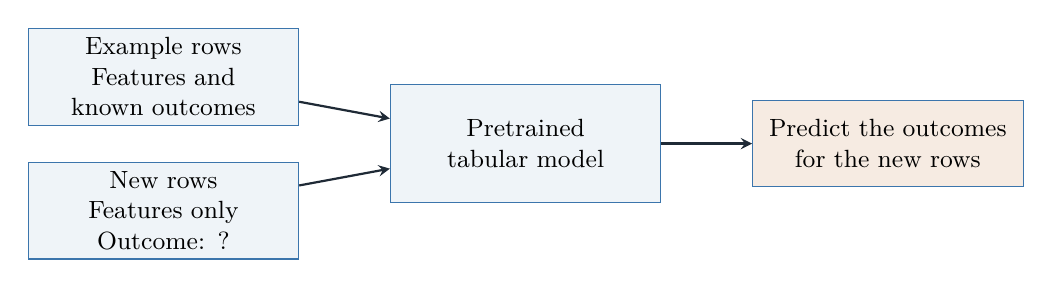
\begin{tikzpicture}[>=stealth,every node/.style={font=\fontsize{9}{11}\selectfont,align=center},
box/.style={draw=MonashBlue,fill=MonashBlue!8,text width=3.2cm,minimum height=1.1cm}]
\node[box] (known) at (0,0) {Example rows\\Features and\\known outcomes};
\node[box] (new) at (0,-1.7) {New rows\\Features only\\Outcome: ?};
\node[box,minimum height=1.5cm] (model) at (4.6,-.85) {Pretrained\\tabular model};
\node[box,fill=Orange!12] (out) at (9.2,-.85) {Predict the outcomes\\for the new rows};
\draw[->,thick](known)--(model);\draw[->,thick](new)--(model);\draw[->,thick](model)--(out);
\end{tikzpicture}
\end{document}
